\begin{frame}{The Sequential Task Flow model}

  \begin{block}{In the Sequential Task Flow (STF) model:}

    \begin{itemize}
    \item The parallel code looks exactly the same as the sequential one
      except that operations are not executed but
      \alert{submitted} to the system in the form of \alert{tasks}
    \item Depending on how tasks access data and on the (sequential) order of submission,
      the runtime infers dependencies among them and builds a DAG
    \item The runtime scheduler deploys the DAG on the
      underlying architecture
    \item The runtime memory manager moves data from one memory to
      another and maintains the global memory coherency
    \item Equivalent to \alert{Superscalar} techniques in microprocessors
    \end{itemize}

  \end{block}

  \vspace{0.2cm}

  Runtimes relying on STF: \alert{StarPU}, QUARK, SMPss, OpenMP 4.0

\end{frame}


\begin{frame}{The STF model: a simple example}

  \begin{columns}
    \begin{column}{0.6\textwidth}
      \begin{block}{Sequential code}
        \texttt{sub\_a(x,y); \gn{// R and W x and y}}\\
        \texttt{sub\_b(x); ~~\gn{// R x} }\\
        \texttt{sub\_c(y); ~~\gn{// R y} }\\
        \texttt{sub\_d(x,y); \gn{// R and W x and y}}\\
      \end{block}

      \vspace{0.5cm}

      \begin{exampleblock}{Equivalent STF code}
        \uncover<2->{\texttt{\alert{submit}(sub\_a,x:\alert{RW},y:\alert{RW});}}

        \uncover<3->{\texttt{\alert{submit}(sub\_b,x:\alert{R});              }}

        \uncover<4->{\texttt{\alert{submit}(sub\_c,y:\alert{R});              }}

        \uncover<5->{\texttt{\alert{submit}(sub\_d,x:\alert{RW},y:\alert{RW});}}

        \uncover<6->{\texttt{\alert{wait\_tasks\_completion}( );}}
      \end{exampleblock}
    \end{column}
    \begin{column}{0.4\textwidth}
      \begin{tikzpicture}[->,>=stealth',shorten >=1pt,auto,node distance=2.8cm,
        semithick]
        \tikzstyle{every state}=[fill=gray,draw=none,text=white]

        \uncover<2->{\node[state]     (A) at (2,5)  {\texttt{sub\_a}};}
        \uncover<3->{\node[state]     (B) at (1,3)  {\texttt{sub\_b}};}
        \uncover<4->{\node[state]     (C) at (3,3)  {\texttt{sub\_c}};}
        \uncover<5->{\node[state]     (D) at (2,1)  {\texttt{sub\_d}};}

        \uncover<3->{\path (A) edge  (B); }
        \uncover<4->{\path (A) edge  (C); }
        \uncover<5->{\path (B) edge  (D); }
        \uncover<5->{\path (C) edge  (D); }
      \end{tikzpicture}
    \end{column}
  \end{columns}

  \vspace{0.5cm}

  \uncover<6->{\texttt{sub\_b} and \texttt{sub\_c} can be executed in \alert{parallel}.}
  \uncover<7->{If \texttt{sub\_a} is executed on CPU and
    \texttt{sub\_b} on GPU, \texttt{x}  will be automatically transferred.}
\end{frame}

\begin{frame}[fragile,t]{The STF parallel multifrontal QR factorization}
  \dr{Sequential} multifrontal $QR$ code with 1D block partitioning

  \begin{columns}[t]
    \begin{column}{0.45\textwidth}
      % \begin{center}
        % 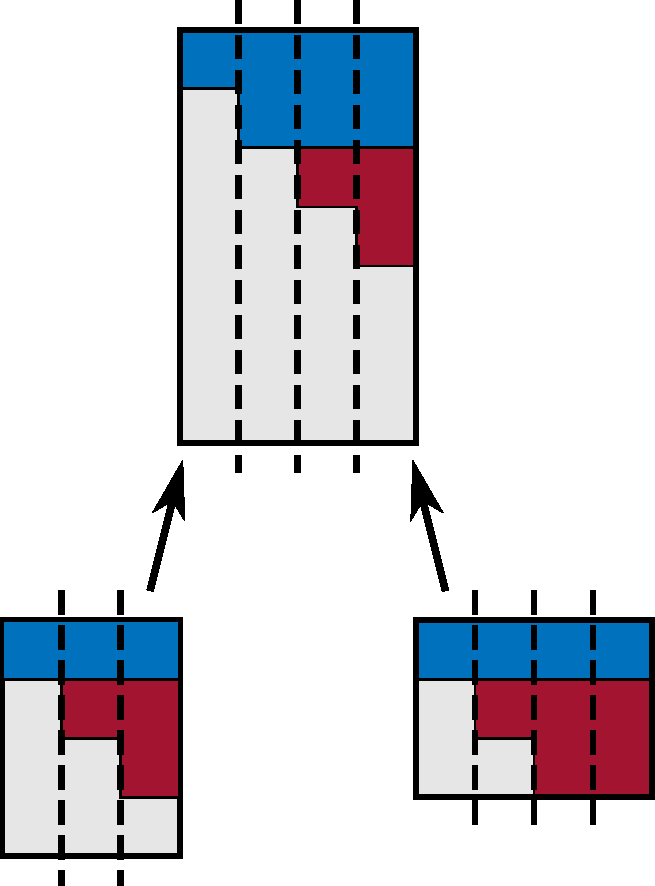
\includegraphics[width=0.6\textwidth]{figures/tree_part}
      % \end{center}
      % \begin{itemize}
      % \item Declare data by registering handles;
      % \item Replace function call with tasks submission;
      % \item Activate operations still performed sequentially;
      % \item Barrier to wait for tasks completion.
      % \end{itemize}
    \end{column}
    \begin{column}{0.55\textwidth}
      \lstinputlisting{listings/mf-seq-multicore.f90}
    \end{column}
  \end{columns}
\end{frame}

\begin{frame}[fragile,t]{The STF parallel multifrontal QR factorization}
  \dr{STF parallel} multifrontal $QR$ code with 1D block partitioning

  \begin{columns}[t]
    \begin{column}{0.45\textwidth}
      % \begin{center}
        % 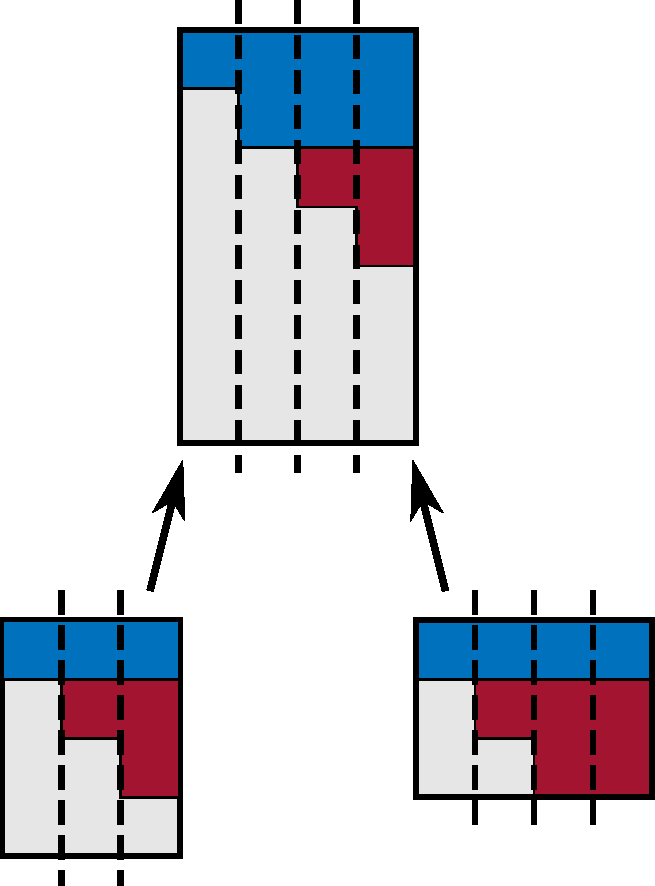
\includegraphics[width=0.6\textwidth]{figures/tree_part}
      % \end{center}
      \begin{itemize}
      \item Declare data by registering handles;
      \item Replace function call with tasks submission;
      \item Activate operations still performed sequentially;
      \item Barrier to wait for tasks completion.
      \end{itemize}
      % \begin{center}
        % 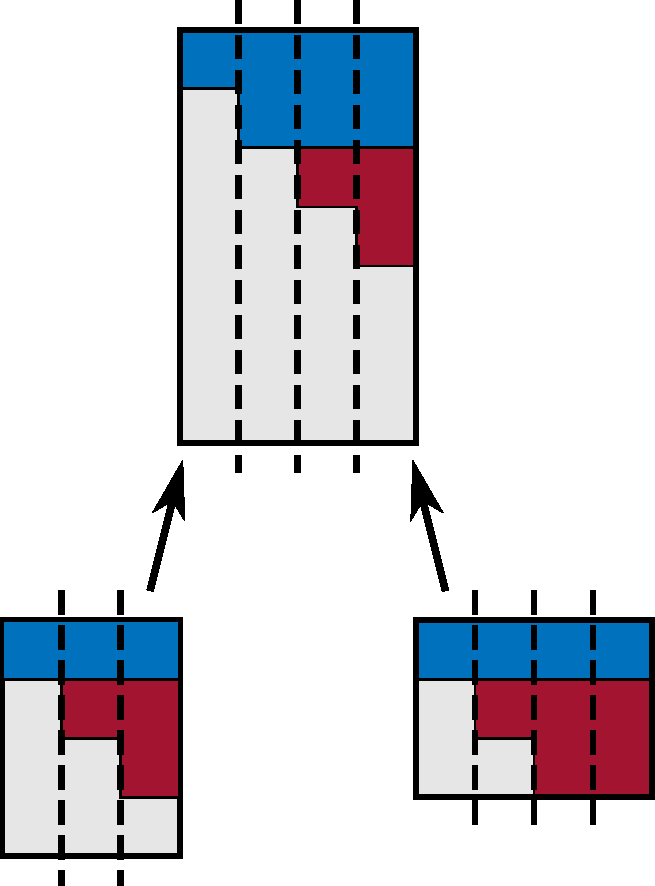
\includegraphics[width=0.6\textwidth]{figures/tree_part}
      % \end{center}
    \end{column}
    \begin{column}{0.55\textwidth}
      \lstinputlisting{listings/mf-stf-multicore.f90}
    \end{column}
  \end{columns}
\end{frame}


\begin{frame}{Experimental results}

  Matrices from the UF SParse Matrix Collection:

  \vspace{0.3cm}

  \begin{center}
    \texttt{\small
      \begin{tabular}{rlrl}
        \hline
        \# & Matrix       & Mflops    & Ordering \\
        \hline
        12 & hirlam       & 1384160   & SCOTCH   \\
        13 & flower\_8\_4 & 2851508   & SCOTCH   \\
        14 & Rucci1       & 5671282   & SCOTCH   \\
        15 & ch8-8-b3     & 10709211  & SCOTCH   \\
        16 & GL7d24       & 16467844  & SCOTCH   \\
        17 & neos2        & 20170318  & SCOTCH   \\
        18 & spal\_004    & 30335566  & SCOTCH   \\
        19 & n4c6-b6      & 62245957  & SCOTCH   \\
        20 & sls          & 65607341  & SCOTCH   \\
        21 & TF18         & 194472820 & SCOTCH   \\
        22 & lp\_nug30    & 221644546 & SCOTCH   \\
        23 & mk13-b5      & 259751609 & SCOTCH   \\
        \hline
      \end{tabular}}
  \end{center}
\end{frame}

\begin{frame}{Experimental results}
  System \db{Ada} (IDRIS supercomputing center):
  \begin{columns}
    \begin{column}{0.5\textwidth}
      % \texttt{\tiny
      %   \begin{tabular}{rlrl}
      %     \hline
      %     \# & Matrix       & Mflops    & Ordering \\
      %     \hline
      %     12 & hirlam       & 1384160   & SCOTCH   \\
      %     13 & flower\_8\_4 & 2851508   & SCOTCH   \\
      %     14 & Rucci1       & 5671282   & SCOTCH   \\
      %     15 & ch8-8-b3     & 10709211  & SCOTCH   \\
      %     16 & GL7d24       & 16467844  & SCOTCH   \\
      %     17 & neos2        & 20170318  & SCOTCH   \\
      %     18 & spal\_004    & 30335566  & SCOTCH   \\
      %     19 & n4c6-b6      & 62245957  & SCOTCH   \\
      %     20 & sls          & 65607341  & SCOTCH   \\
      %     21 & TF18         & 194472820 & SCOTCH   \\
      %     22 & lp\_nug30    & 221644546 & SCOTCH   \\
      %     23 & mk13-b5      & 259751609 & SCOTCH   \\
      %     \hline
      %   \end{tabular}}
        \begin{itemize}
        \item IBM x3750-M4
        \item Intel Sandy Bridge E5-4650 @ 2.7
          GHz, $4\times 8$ cores
        \item 128 GB memory (NUMA)
        \end{itemize}

    \end{column}
    \begin{column}{0.5\textwidth}
        
        \begin{itemize}
        \item Compilers Intel ifort and icc 15.0.2
        \item BLAS and LAPACK libraries from Intel MKL 11.2.
        \end{itemize}
    \end{column}
  \end{columns}

  \begin{center}
    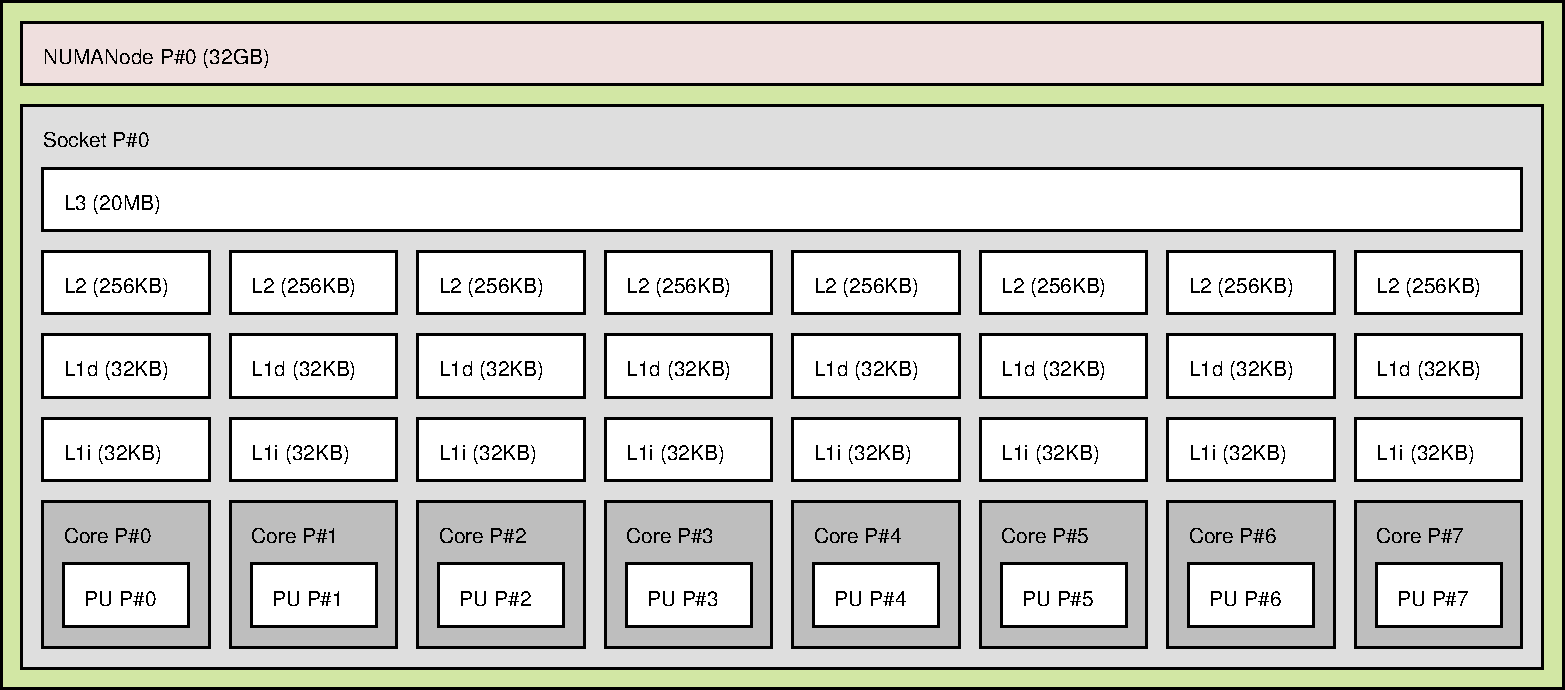
\includegraphics[width=0.8\textwidth]{figures/ada}
  \end{center}
    
\end{frame}

\begin{frame}{Experimental results: speedups}
  \begin{center}
    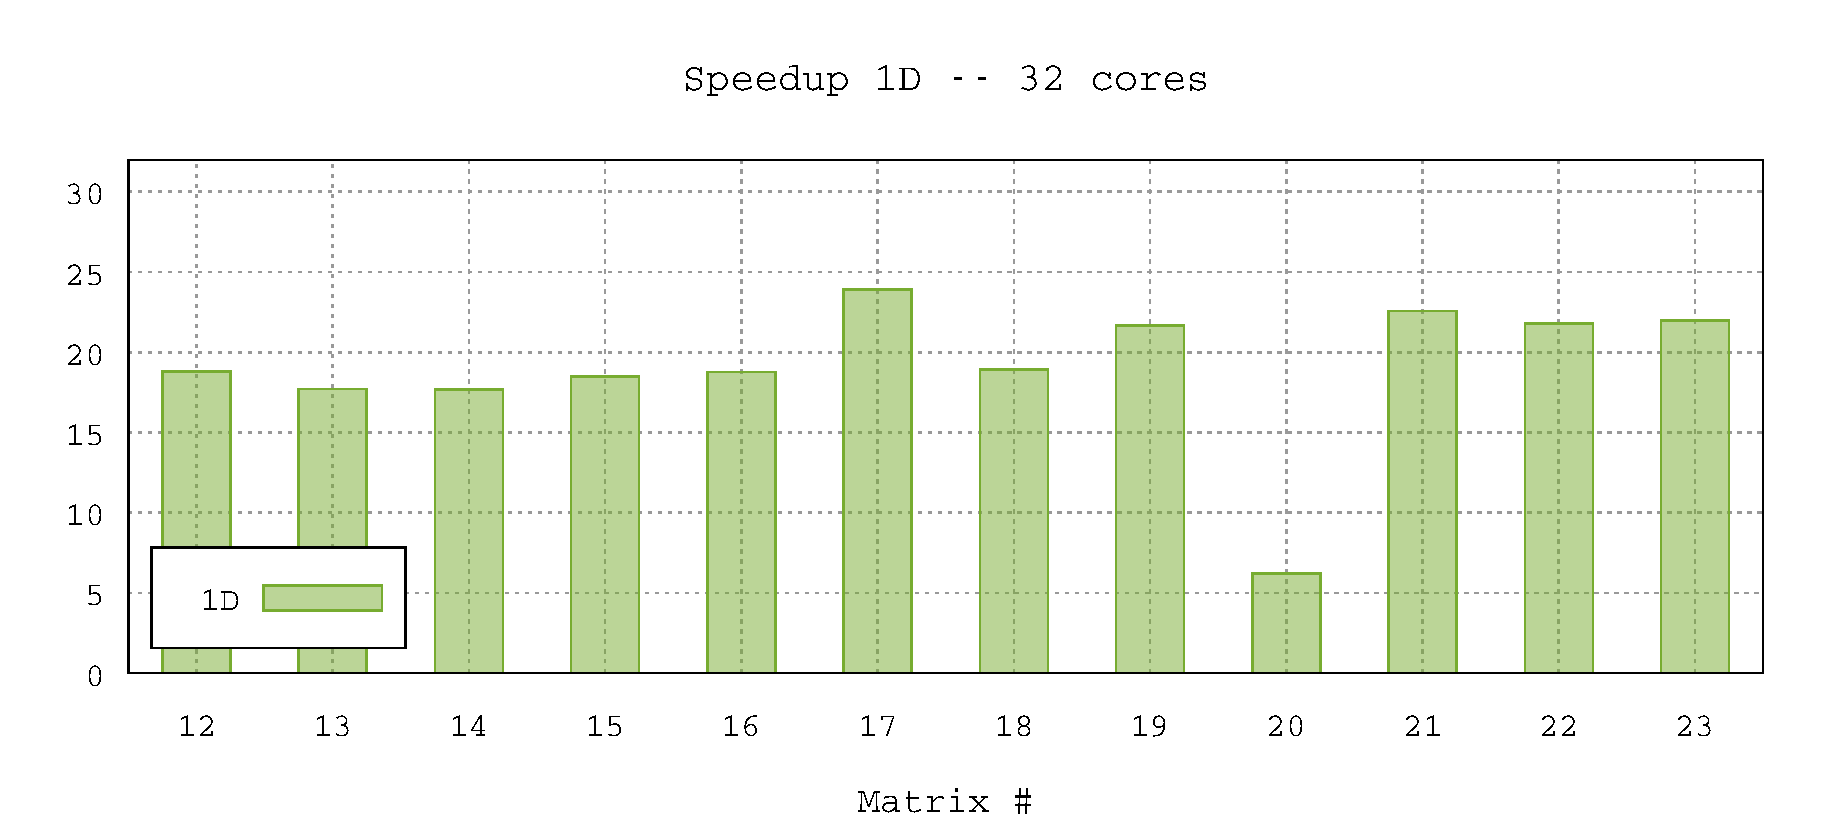
\includegraphics[width=0.9\textwidth]{data/su_ada_toms_1d}
  \end{center}
  
  The task-based multifrontal method, implemented with a STF parallel
  model on top of \starpu offers good speedups on 32 cores:

  \begin{itemize}
  \item speedup increases with problem size with very low speedup for
    some problem such as matrix \# 20
  \item we use a detailed performance analysis to determine the
    limiting factors of the STF 1D approach
  \end{itemize}

\end{frame}

\begin{frame}{Area performance upper bound}


  \begin{block}{Parallel efficiency}
    The \dr{parallel efficiency} is defined as
    
    \begin{displaymath}
      e(p) = \frac{\tilde{t}(1)}{t(p)\cdot p}
    \end{displaymath}
    
    \begin{itemize}
    \item $\tilde{t}(1)$ is the execution time of the \alert{best
        sequential algorithm} on one core;
    \item $t(p)$ is the execution time of the \alert{best parallel
        algorithm} on $p$ cores.
    \end{itemize}
  \end{block}
    
    \vspace{0.2cm}
    
  Note that, in general, $t(1) \ge \tilde{t}(1)$ because:
  \begin{itemize}
  \item parallelism requires partitioning of data and operations which
    reduces the efficiency of tasks;
  \item the parallel algorithm may trade some extra flops for
    concurrency.
  \end{itemize}


\end{frame}


% \begin{frame}{Area performance upper bound}

%   The \dr{parallel efficiency} can be defined as

%   \begin{displaymath}
%     e(p) = \frac{t^{min}(p)}{t(p)}
%   \end{displaymath}

%   where \dr{$t^{min}(p)$} is a lower bound on execution time on $p$  resources:
%   % resources corresponding to the \alert{best schedule} under the
%   % following assumptions:

%   % \begin{columns}
%   %   \begin{column}{0.45\textwidth}

%   %     \begin{enumerate}
%   %     \item<2-> No runtime overhead.
%   %     \item<3-> No tasks dependencies.
%   %     \item<4-> Tasks are moldable.
%   %       %% \item<2-> Tasks executed at asymptotic performance (\alert{maximum task granularity})
%   %       %% \item<2-> \alert{Perfect data locality}
%   %     \end{enumerate}

%   %   \end{column}
%   %   \begin{column}{0.55\textwidth}

%   %     \begin{center}
%   %       \only<1 >{\includegraphics[width=\textwidth]{lp_anim_mul2}}%
%   %       \only<2 >{\includegraphics[width=\textwidth]{lp_anim_mul3}}%
%   %       \only<3 >{\includegraphics[width=\textwidth]{lp_anim_mul4}}%
%   %       \only<4->{\includegraphics[width=\textwidth]{lp_anim_mul5}}%
%   %     \end{center}

%   %   \end{column}
%   % \end{columns}
      
%   \begin{itemize}
%   \item<2-> In the multicore case (homogeneous) we have 

%     \begin{displaymath}
%       t^{min}(p) = \frac{t(1) }{ p }
%     \end{displaymath}

%   \item<3-> We consider \dr{$t^{min}(p)$} when there is no performance
%     loss resulting from the parallelization
%     \dr{$\tilde{t}^{min}(p)$}. In the multicore case we have
    
%     \begin{displaymath}
%       \tilde{t}^{min}(p) = \frac{ \tilde{t}(1) }{ p }
%     \end{displaymath}

%   \end{itemize}

% \end{frame}


\begin{frame}{A finer performance analysis}
  The execution time $t(p)$ can be decomposed in the following three
  terms:
  \begin{itemize}
  \item \db{$t_t(p)$}: the time spent executing tasks.
  \item \mye{$t_r(p)$}: the overhead of the runtime system. \alert{$t_r(1):=0$}.
  \item \dg{$t_i(p)$}: idle time. \alert{$t_i(1):=0$}.
  \end{itemize}

  The overall efficiency can thus be written as:
  

  % \begin{displaymath}
    % e(p) = \frac{ \tilde{t}_t(1) }{ t_t(p) + t_r(p) + t_i(p) }
  % \end{displaymath}
  
  % \begin{displaymath}
    % = \mre{\overbracket{\mbk{\frac{ \tilde{t}_t(1) }{ t_t(1) }}}^{e_g}}\cdot 
    % \mbl{\overbracket{\mbk{\frac{ t_t(1) }{ t_t(p) }}}^{e_{t}}}\cdot  
    % \mgr{\overbracket{\mbk{\frac{ t_t(p) }{ t_t(p)+t_r(p) }}}^{e_r}}\cdot
    % \mye{\overbracket{\mbk{\frac{ t_t(p)+t_r(p)+ t_c(p) }{ t_t(p) + t_r(p) + t_c(p) + t_i(p) }}}^{e_p}}.
  % \end{displaymath}
  


\begin{align*}
  e(p) & = \frac{ \tilde{t}_t(1) }{ t_t(p) + t_r(p) + t_i(p) } \\
       & = \mre{\overbracket{\mbk{\frac{ \tilde{t}_t(1) }{ t_t(1) }}}^{e_g}}\cdot 
  \mbl{\overbracket{\mbk{\frac{ t_t(1) }{ t_t(p) }}}^{e_{t}}}\cdot  
  \mye{\overbracket{\mbk{\frac{ t_t(p) }{ t_t(p)+t_r(p) }}}^{e_r}}\cdot
  \mgr{\overbracket{\mbk{\frac{ t_t(p)+t_r(p)+ t_c(p) }{ t_t(p) + t_r(p) + t_c(p) + t_i(p) }}}^{e_p}}.
\end{align*}

    % \begin{displaymath}
    %   \tiny
    %     e(p) = \mbk{\frac{\tilde{t}^{area}(p)}{t(p)}} 
    %     % = \frac{ \tilde{t}^{area}(p) \times p }{ t_t(p) + t_r(p) + t_c(p) + t_i(p) } = \frac{ \tilde{t}^{area}_t(p) }{ t_t(p) + t_r(p) + t_c(p) + t_i(p) }
    %     = \mre{\overbracket{\mbk{\frac{ \tilde{t}^{area}_t(p) }{ t^{area}_t(p) }}}^{e_g}}\cdot
    %     \mbl{\overbracket{\mbk{\frac{ t^{area}_t(p) }{ t_t(p) }}}^{e_{t}}}\cdot
    %     \mgr{\overbracket{\mbk{\frac{ t_t(p) }{ t_t(p)+t_r(p) }}}^{e_r}}\cdot
    %     \mbp{\overbracket{\mbk{\frac{ t_t(p)+t_r(p) }{t_t(p)+t_r(p)+ t_c(p)}}}^{e_c}}\cdot
    %     \mye{\overbracket{\mbk{\frac{ t_t(p)+t_r(p)+ t_c(p) }{ t_t(p) + t_r(p) + t_c(p) + t_i(p) }}}^{e_p}}.
    % \end{displaymath}

%   \begin{displaymath}
% e(p) = \frac{t^{area}(p)}{t(p)} =%
% \only<1,3,4,5>{\overbracket{\frac{t^{area}_t(p)}{t_t(p)}}^{e_h}}%
% \only<2>{\dr{\overbracket{\frac{t^{area}_t(p)}{t_t(p)}}^{e_h}}}%
% \cdot%
% \only<1,2,4,5>{\overbracket{\frac{t_t(p)}{t_t(p)+t_r(p)}}^{e_r}}%
% \only<3>{\dg{\overbracket{\frac{t_t(p)}{t_t(p)+t_r(p)}}^{e_r}}}%
% \cdot%
% \only<1,2,3,5>{\overbracket{\frac{t_t(p)+t_r(p)}{t_t(p)+t_r(p)+t_i(p)}}^{e_p}}%
% \only<4>{\db{\overbracket{\frac{t_t(p)+t_r(p)}{t_t(p)+t_r(p)+t_i(p)}}^{e_p}}}%
%   \end{displaymath}
  
  \vspace{0.5cm}

  with:

  \vspace{0.3cm}

  \begin{overlayarea}{\textwidth}{3cm}
    \only<2>{\dr{$e_g$}: the \dr{granularity efficiency}. Measures the
      impact exploiting of parallel algorithms compared to sequential
      ones.}%
    \only<3>{\db{$e_t$}: the \db{task efficiency}. Measures the
      exploitation of data locality.}%
    \only<4>{\mye{$e_r$}: the \mye{runtime efficiency}. Measures how the
      runtime overhead affects performance.}%
    \only<5>{\dg{$e_p$}: the \dg{pipeline efficiency}. Measures how
      much concurrency is available and how well it is exploited.}%
    % \begin{itemize}
    % \item<5> if $e_h>1$ GPUs are overloaded and CPU starve ($e_p<1$)
    % \item<5> if $e_h<1$ tasks acceleration factor not properly exploited
    % \end{itemize}%

    % \only<7>{$e_t \cdot e_p$ measures the quality of the scheduling
    % and is $\leq 1$.}
  \end{overlayarea}

\end{frame}

\begin{frame}{Experimental results: efficiency breakdown}
  \centering
  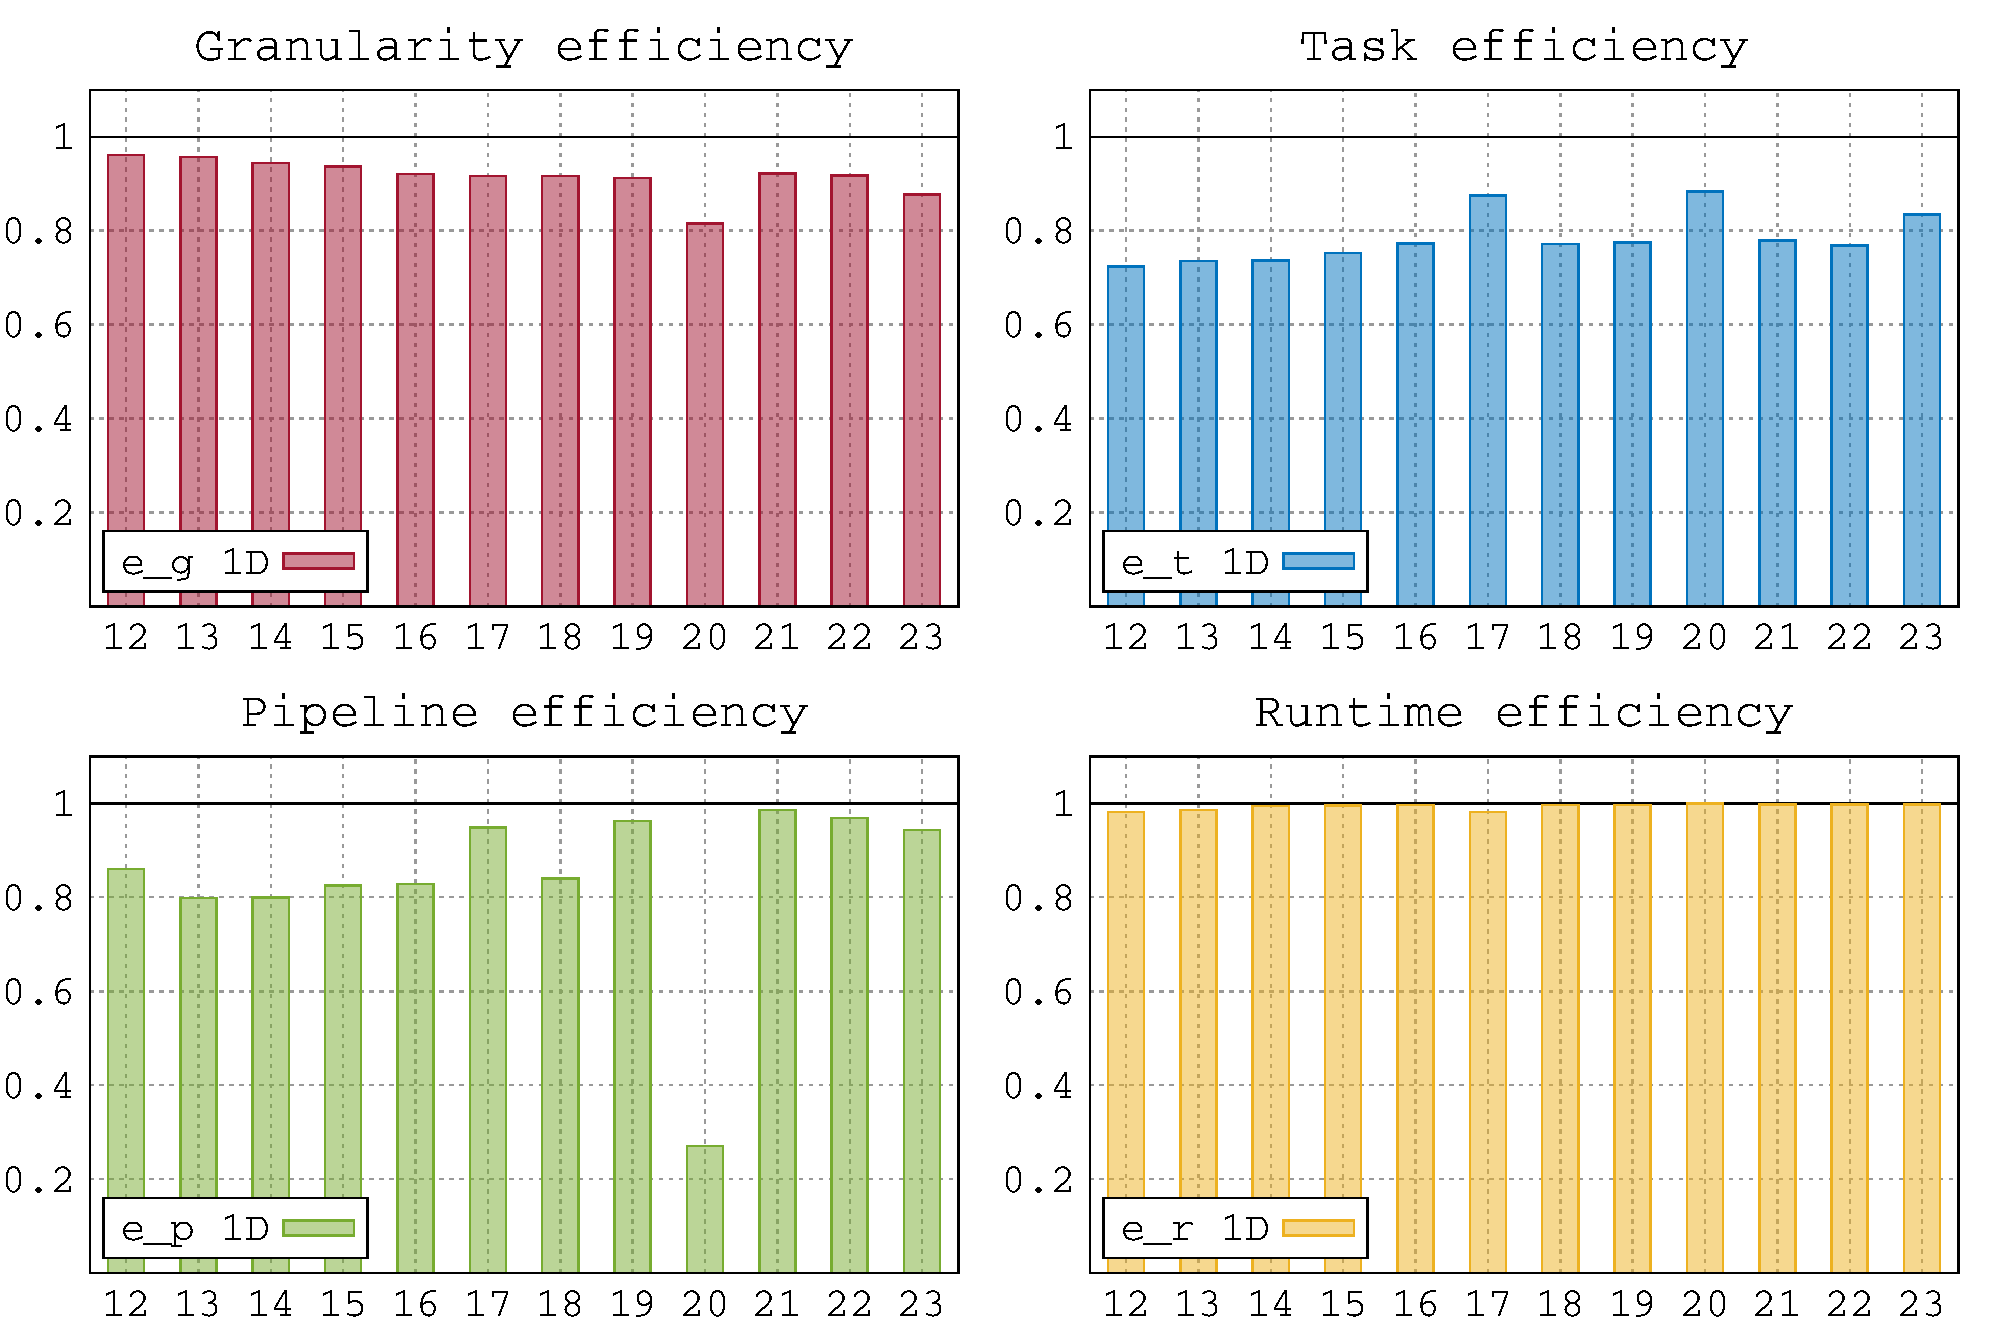
\includegraphics[width=\textwidth]{data/eff_profiles_2x2_1d}
\end{frame}

\begin{frame}{2D partitioning + CA front factorization}
  1D partitioning is not good for (strongly)
  \db{overdetermined} matrices:
  \begin{itemize}
  \item[\dr{$\blacktriangledown$}] Most fronts are overdetermined
  \item[\dg{$\blacktriangle$}] The problem is mitigated by
    concurrent front factorizations
  \end{itemize}


  \begin{columns}
    \begin{column}{0.8\textwidth}
      \begin{itemize}
      \item 2D block partitioning (not necessarily square)
        %% \item flat, binary (communication avoiding) or hybrid panel
        %%   reduction trees
      \item Communication avoiding algorithms
      \item[\dg{$\blacktriangle$}] More concurrency
      \item[\dr{$\blacktriangledown$}] More complex dependencies
      \item[\dr{$\blacktriangledown$}] Many more tasks (higher runtime overhead)
      \item[\dr{$\blacktriangledown$}] Finer task granularity (less kernel efficiency)
      \end{itemize}
      Thanks to the simplicity of the STF programming model it is
      possible to plug in \alert{2D methods} for factorizing the frontal
      matrices with a relatively moderate effort
    \end{column}
    \begin{column}{0.2\textwidth}
      \begin{center}
        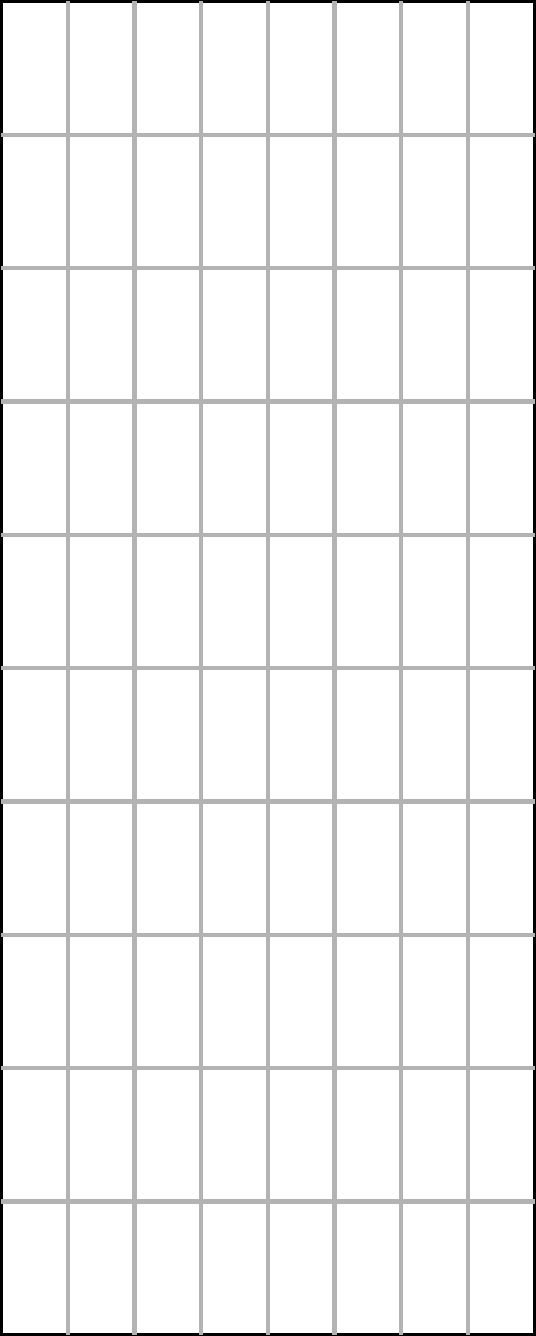
\includegraphics[width=\textwidth]{figures/2d}
      \end{center}
    \end{column}
  \end{columns}
\end{frame}

\begin{frame}[t,plain,fragile]{1D partitioning front factorization}
  \lstinputlisting{listings/mf-stf-multicore.f90}
\end{frame}

\begin{frame}[t,plain,fragile]{2D partitioning + CA front factorization}
  \lstinputlisting{listings/mf-stf-2d-multicore.f90}
\end{frame}

\begin{frame}{Experimental results: speedups}

  \begin{center}
    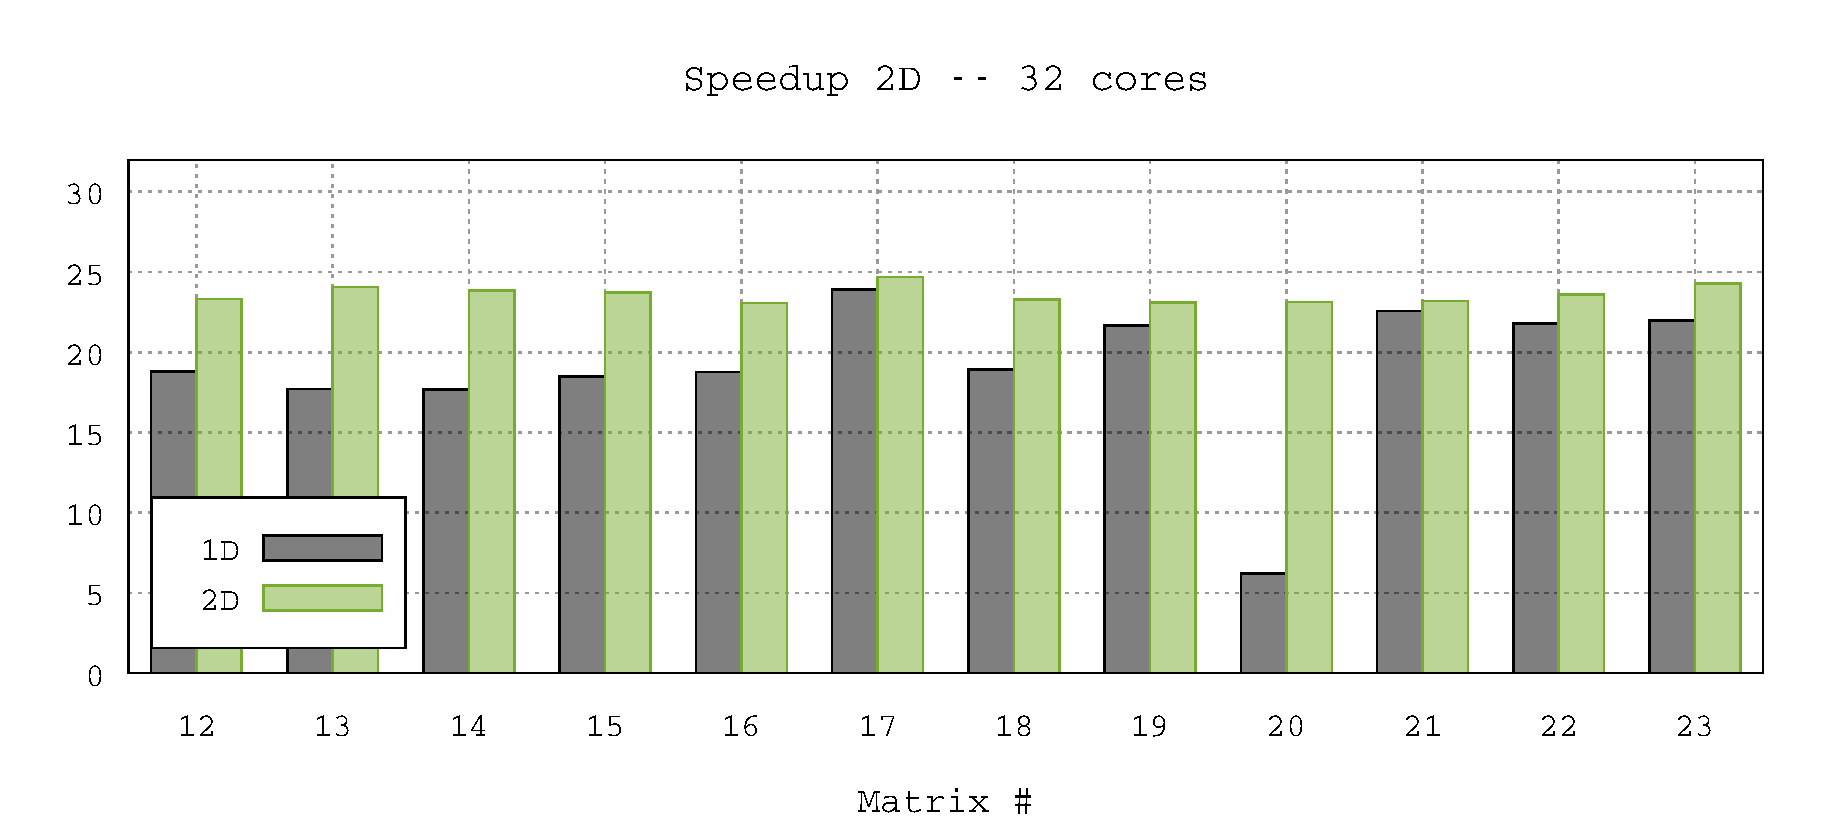
\includegraphics[width=0.9\textwidth]{data/su_ada_toms_2d}
  \end{center}

  The scalability of the task-based multifrontal method is enhanced by
  the the introduction of 2D CA algorithms:

  \begin{itemize}
  \item Speedups are \dr{uniform} for all tested matrices.
  \item We perform a comparative performance analysis wrt to the 1D
    case to show the benefits of the 2D scheme. 
  \end{itemize}

\end{frame}

\begin{frame}{Experimental results: efficiency breakdown}
  \centering
  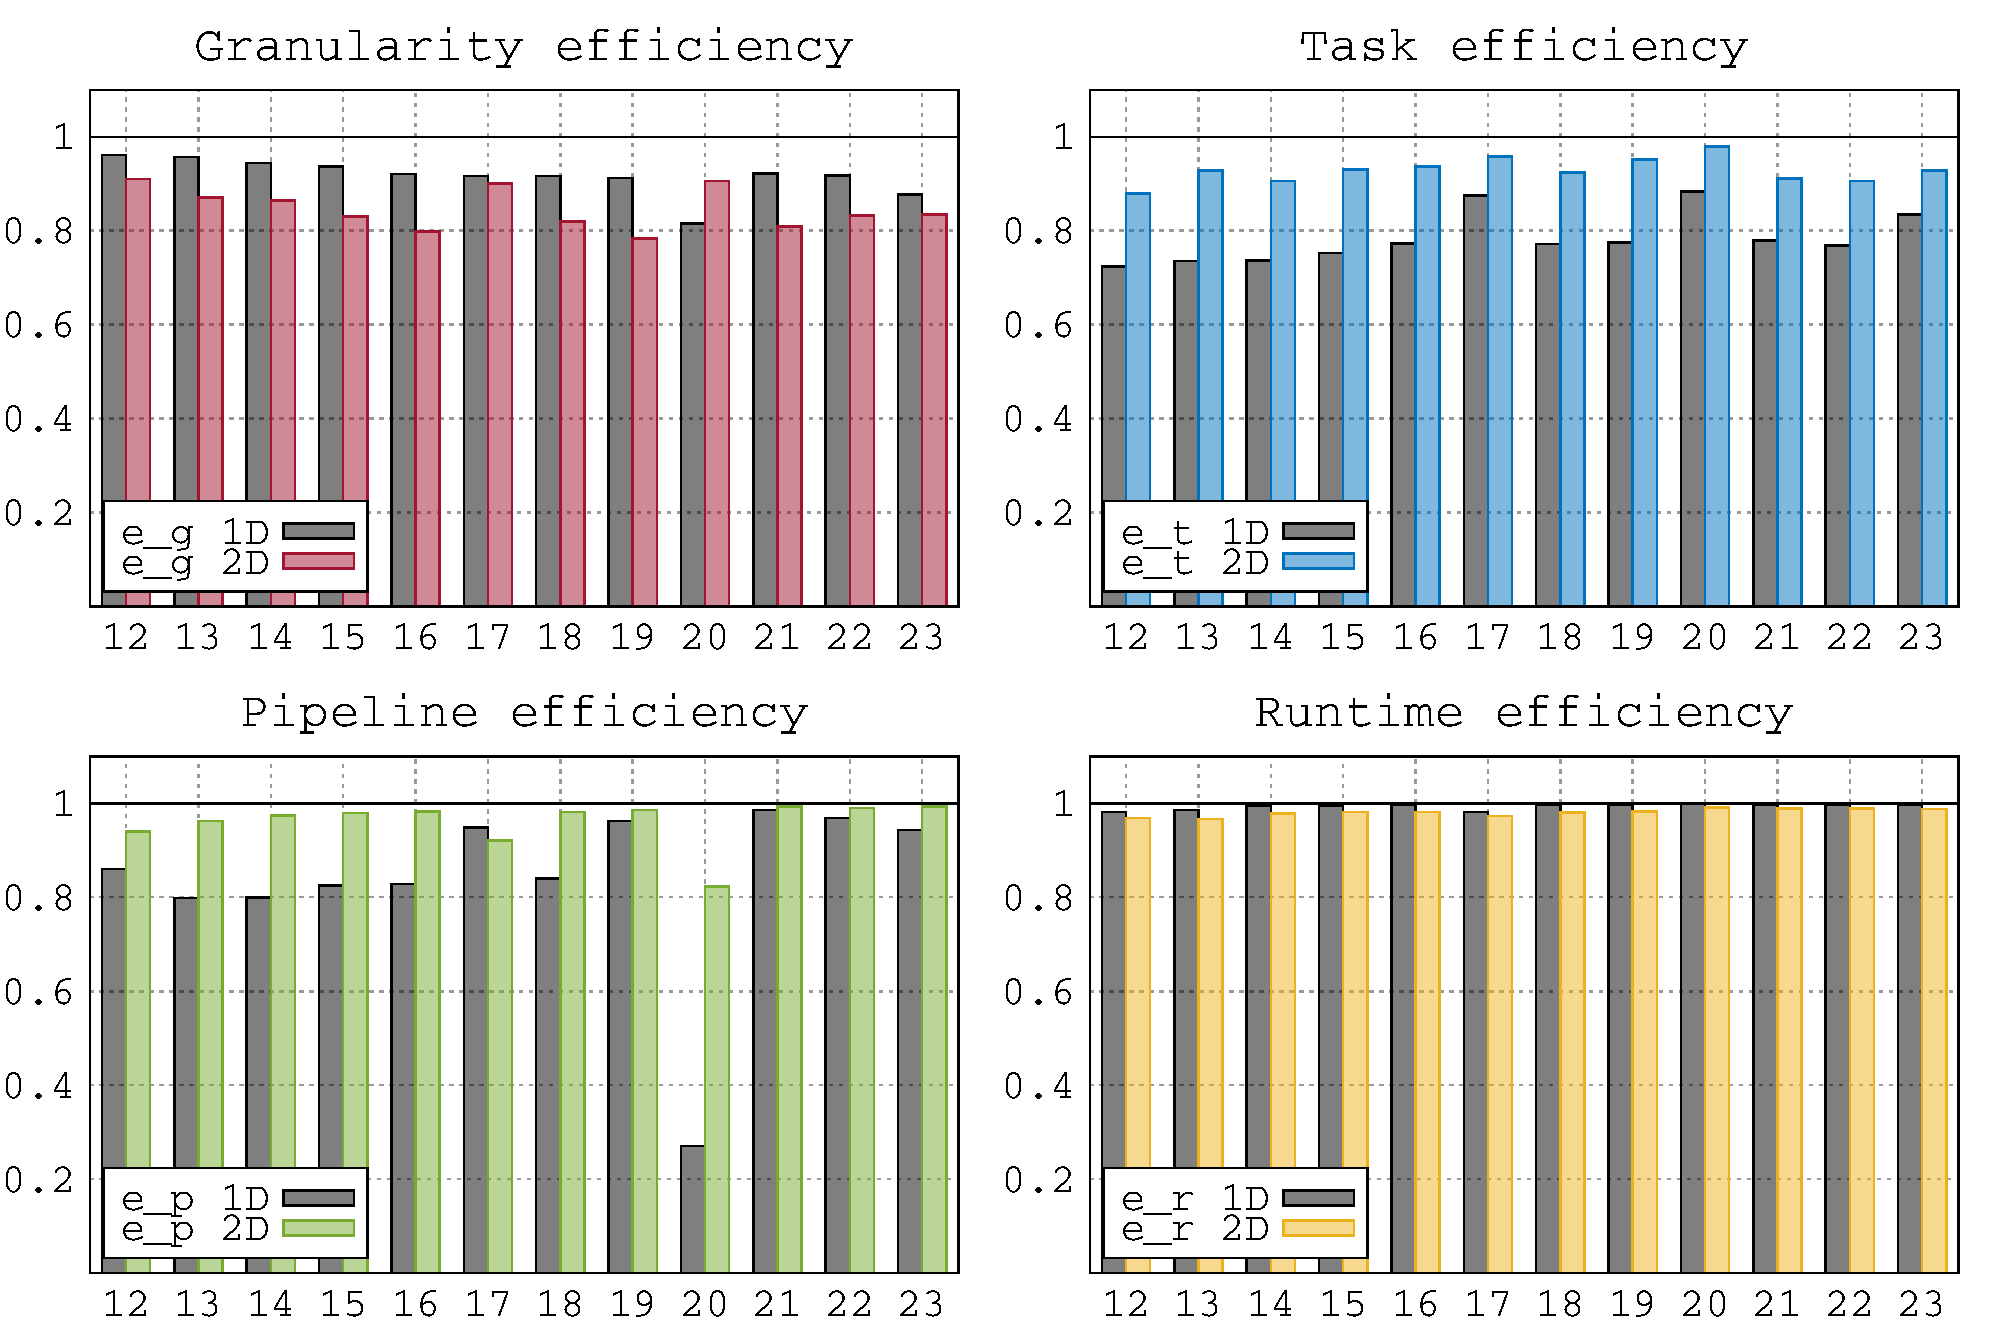
\includegraphics[width=\textwidth]{data/eff_profiles_2-2_2d}
\end{frame}

%%% Local Variables:
%%% mode: latex
%%% TeX-master: "defense"
%%% TeX-engine: xetex
%%% End:
